%% This is going to be my carbon nanotube chapter. It should be based almost completely on GBO notes

\chapter{Electronic Properties of Carbon Nanotubes}
\label{sec:CNT}
\chaptermark{Properties of CNTs}

Carbon nanotubes exhibit a variety of interesting material and electrical properties. Nanotubes can be used as mechanical oscillators, one dimensional conductors, and quantum dots, among many other applications. The work in this thesis takes advantage of the unique electronic and spin transport properties of carbon nanotubes. By starting with the graphene lattice, these properties are easily derived. 

\section{Electronic Bandstructure of Graphene}

The electronic bandstructure of graphene was first calculated in 1947 by P.R. Wallace (CITE). This was done as part of an effort to understand the electronic structure of bulk graphite. In this paper, there is mention of the two lowest energy bands and the half filling of a single layer of carbon atoms. It was not until 1984 that Semenoff discussed the existence of a linear dispersion relation for low energy electronic excitations in single layers of carbon atoms (CITE). This was done by looking at a generic honeycomb lattice as an analoge of 2+1 dimensional electrodynamics. Semenoff found the low energy electronic band structure of the monoatomic honeycomb lattice matched that of Dirac fermions.

Graphene was first isolated on silicon wafers through mechanical exfoliation in 2004. The semimetallic characteristics were confirmed through measuring transistor curves and the charge carrier sign change through the Hall effect (CITE). Shortly after, the same research group confirmed the existance of low energy Dirac fermions in graphene (CITE).

Beginning with the structure of the monoatomic honeycomb lattice, and following the original work of Wallace, the electronic band structure of graphene will be derived below.

\subsection{Graphene Lattice}

As mentioned above, single layers of carbon atoms, graphene, form a honeycomb lattice. This lattice can be seen in Figure \ref{fig:graphene_unit_cell}.

\begin{figure}
    \centering
    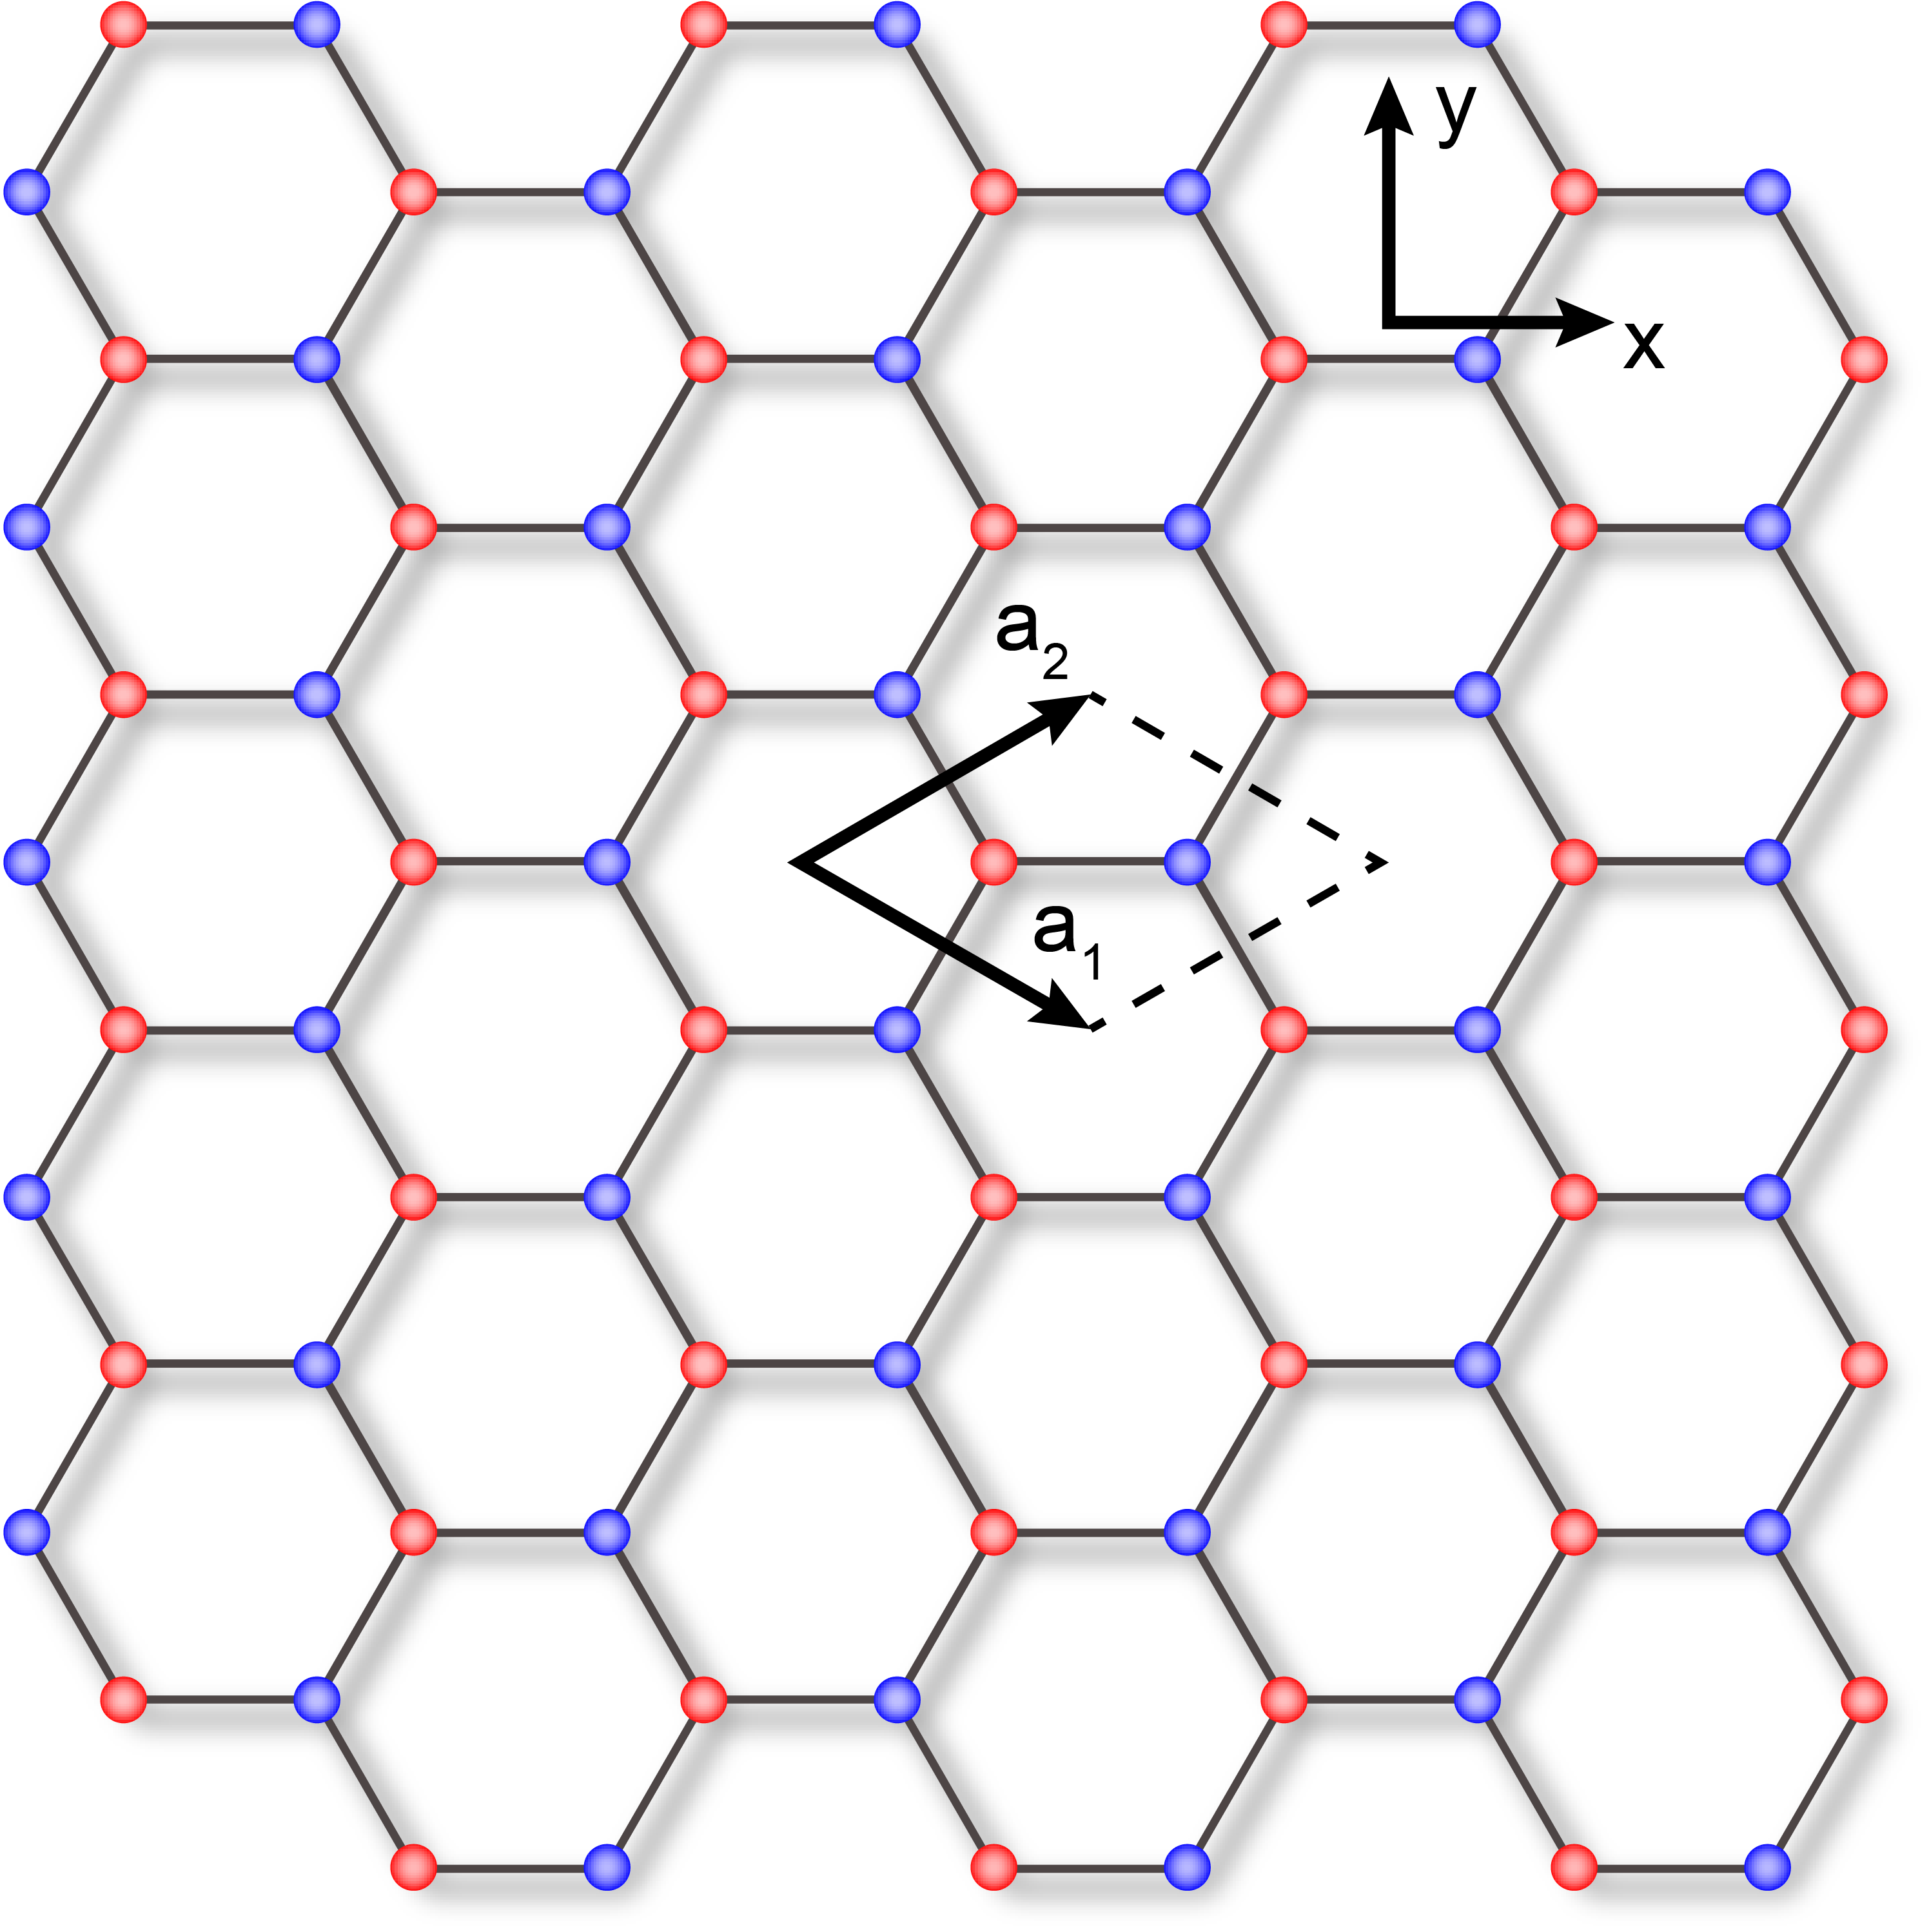
\includegraphics[width = 0.5\textwidth]{chapter2/graphene_unit_cell.png}
    \caption{The real-space structure of the graphene lattice. Vectors $\vec{a}_1$ and $\vec{a}_2$ define the unit cell, which contains two atoms, highlighted in red and blue.}
    \label{fig:graphene_unit_cell}
\end{figure}

In Figure \ref{fig:graphene_unit_cell} the unit cell is defined by the two lattice vectors $\vec{a}_1$ and $\vec{a}_2$. Each unit cell is comprised of two atoms. The honeycomb lattice can be thought of as to interpenetrating triangular sublattices. With that picture, the honeycomb unit cell contains one atom from each of the two sublattices, highlighted in Figure \ref{fig:graphene_unit_cell} as red (A) and blue (B). Each atom on the lattice contributes one conduction electron.

Using the coordinates defined in Figure \ref{fig:graphene_unit_cell}, the lattice vectors are defined, from the center of a honeycomb.

\begin{align}
    \vec{a}_1 &= \frac{3a_0}{2}\hat{i} + \frac{\sqrt{3}a_0}{2}\hat{j} \\
    \vec{a}_2 &= \frac{3a_0}{2}\hat{i} - \frac{\sqrt{3}a_0}{2}\hat{j}
\end{align}

Here $a_0$ is the carbon-carbon bond distance, \SI{1.42}{\angstrom} (CITE).

The reciprocal lattice vectors, $\vec{b}_1$ and $\vec{b}_2$ can now be found in the usual way.

\begin{equation}
    a_i \cdot b_j = 2\pi \delta_{ij}
\end{equation}

Here $\delta_{ij}$ is the Kronecker delta. The reciprocal lattice defined by $\vec{b}_1$ and $\vec{b}_2$ can be seen in Figure \ref{fig:graphene_k_space}.

\begin{align}
    \vec{b}_1 &= \frac{2\pi}{3a_0}\hat{i} + \frac{2\sqrt{3}\pi}{3a_0}\hat{j} \\
    \vec{b}_2 &= \frac{2\pi}{3a_0}\hat{i} - \frac{2\sqrt{3}\pi}{3a_0}\hat{j}
\end{align}

\begin{figure}
    \centering
    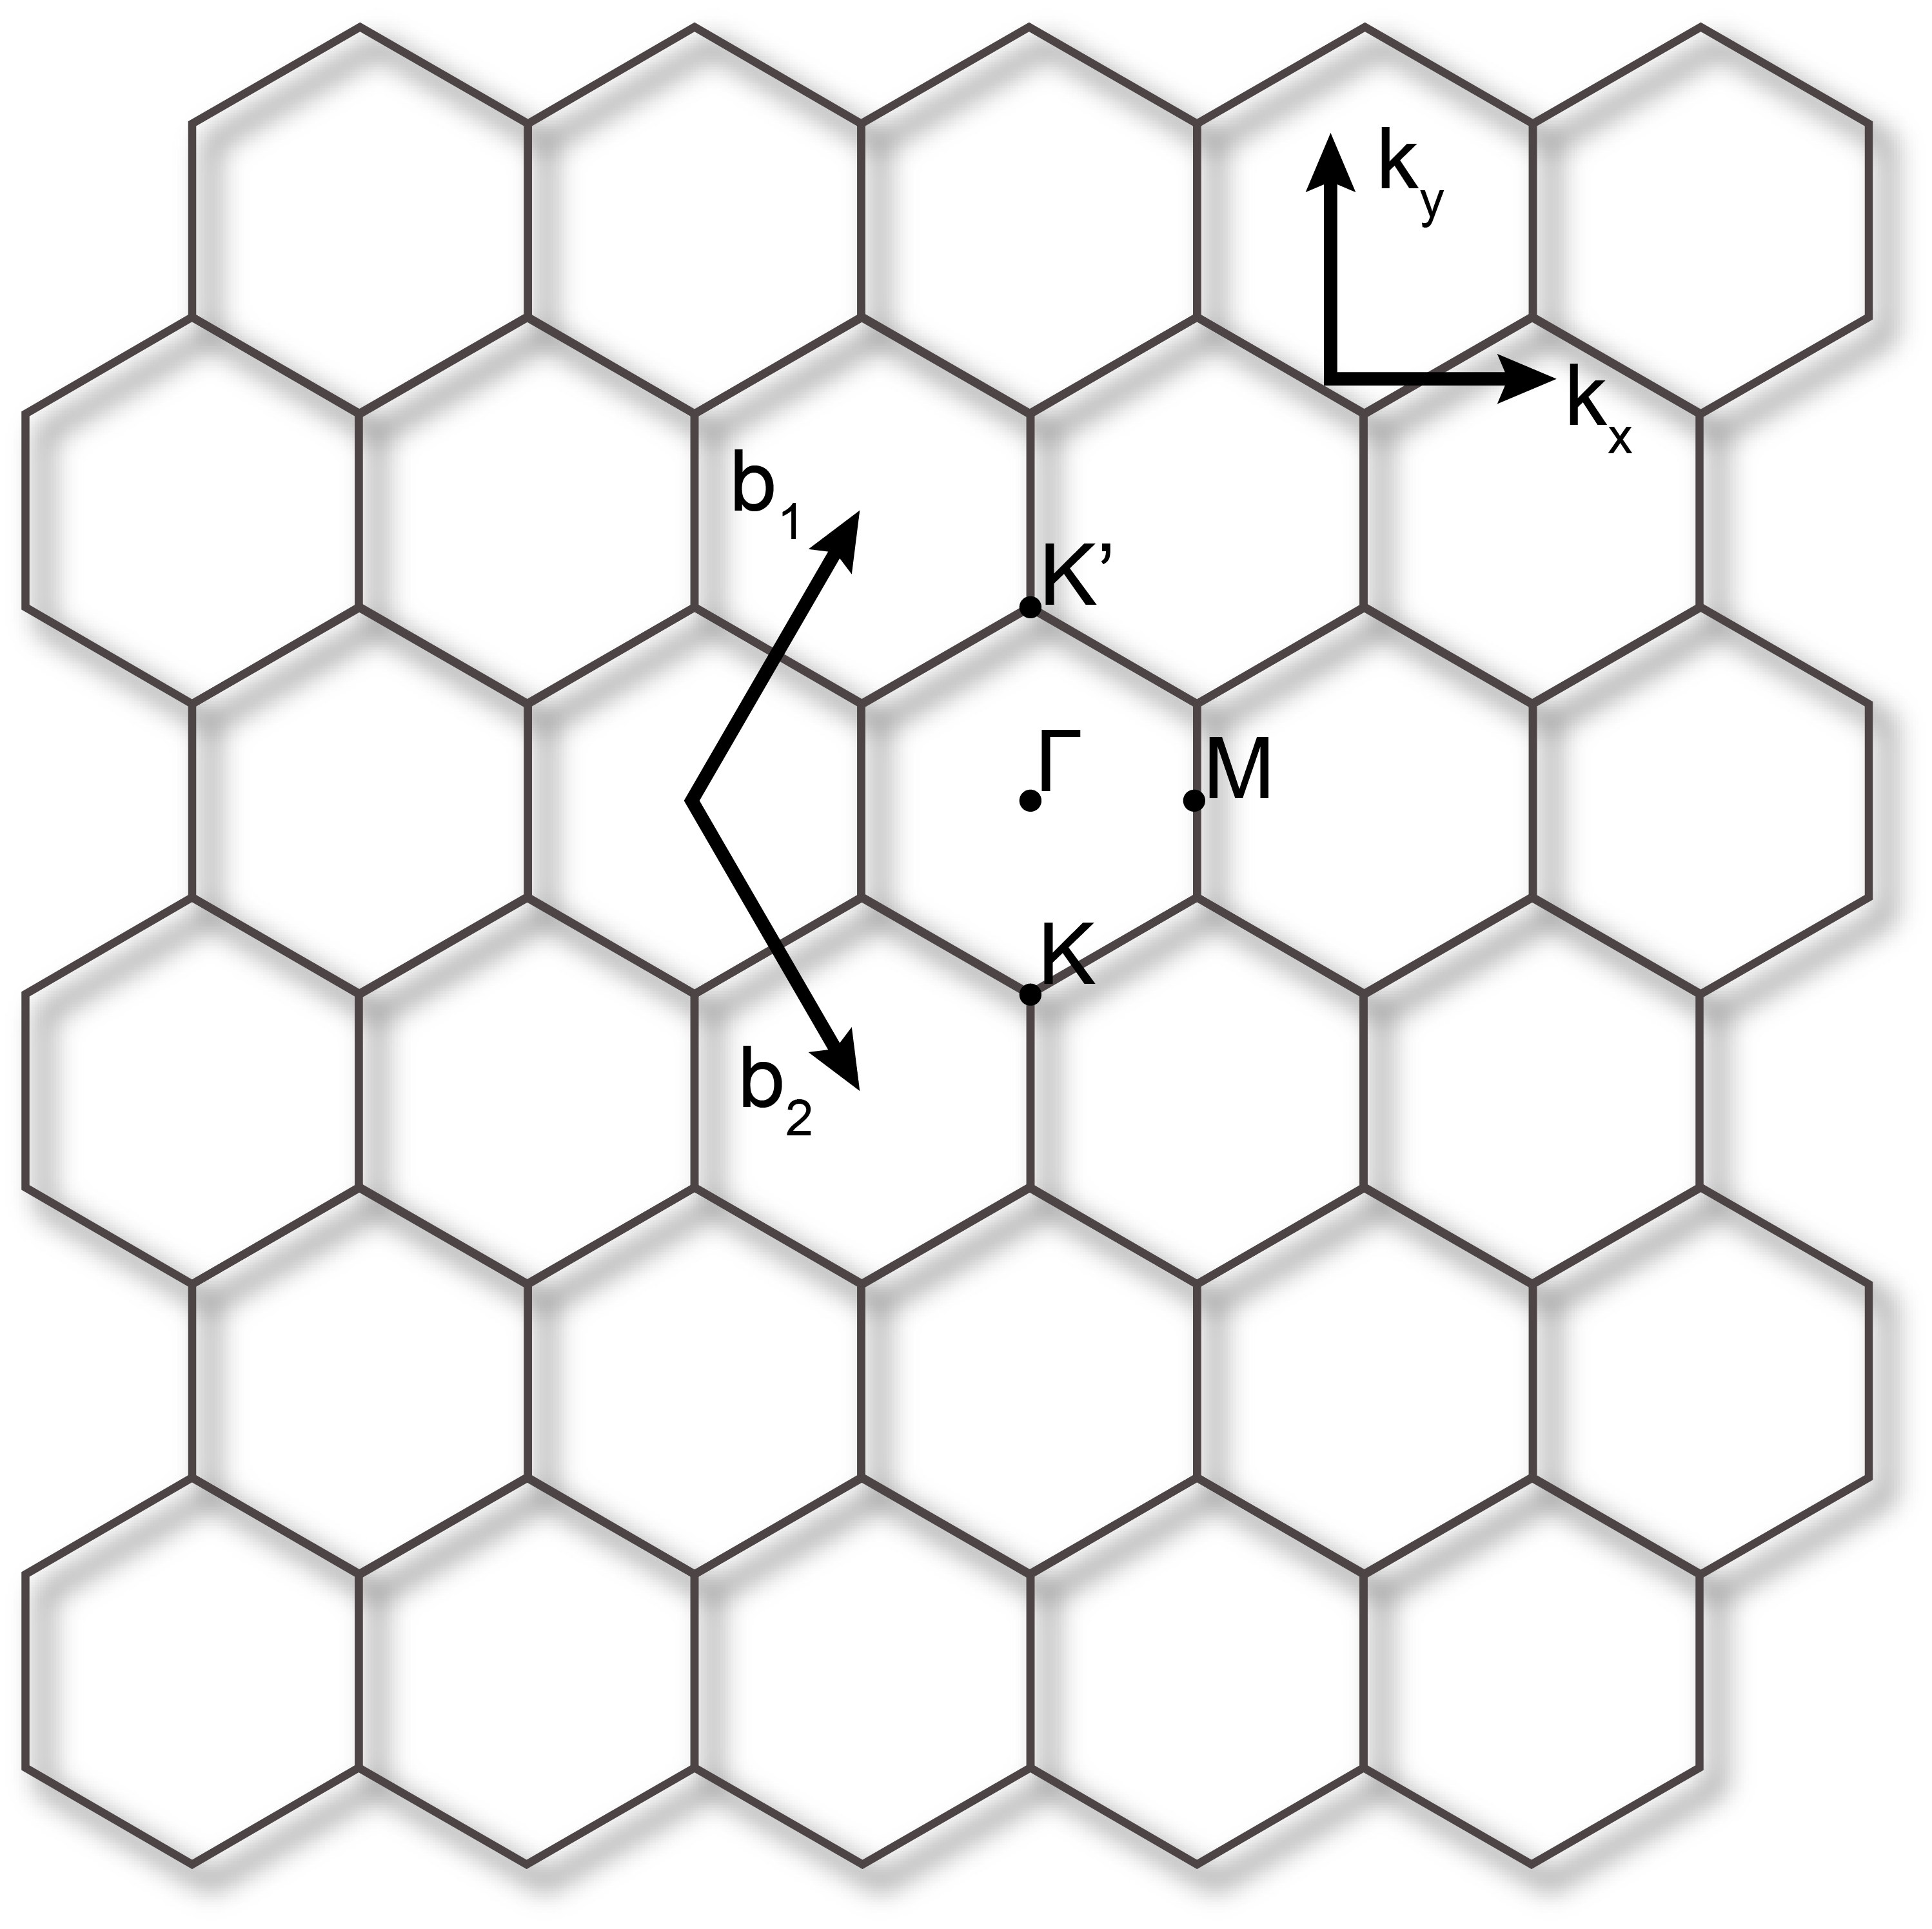
\includegraphics[width = 0.5\textwidth]{chapter2/graphene_k_space.png}
    \caption{The reciprocal lattice of graphene. Vectors $\vec{b}_1$ and $\vec{b}_2$ define the Brillouin zone. The high symmetry points $\Gamma$, $K$, $K'$, and $M$ are labeled.}
    \label{fig:graphene_k_space}
\end{figure}

The reciprocal lattice is also a honeycomb lattice, rotated 90 degrees from the real space lattice. The size of each Brillouin zone is defined by the reciprocal lattice vectors above. A few high symmetry points have been labelled in the figure. Of particular note are the three $K$ and three $K'$ points. As will be seen in the band structure calculation, these are the points at which the conduction and valence bands will meet to form the Dirac cones that give rise to graphene's interesting low energy conduction properties.

\subsection{Tight Binding Model}

The simplest way to calculate the low energy electronic band structure for graphene is using a nearest neighbor tight binding model, also known as a linear combination of atomic orbitals (CITE). In this model, each conduction electron is tightly bound to a lattice site with a small probability of hopping only to a nearest neighbor site. With this simple picture for electron conduction, one can find the lowest energy bands in graphene.

Given that the model deals with the motion of individual electrons and their wavefunctions at each atomic site, the goal will be to solve the time independent Schr\"{o}dinger equation.

\begin{equation}
    \hat{H}\Psi = \varepsilon\Psi
\end{equation}

$\Psi$ is a single particle wavefunction over the whole graphene lattice. As such, it can be written as a linear combination of Bloch wavefucntions.

\begin{align}
    u_A(\vec{r}) &= \frac{1}{\sqrt{N}}\sum_{\vec{r}_A}^{} e^{i\vec{k}\cdot\vec{r}_A} \phi_{2p_z}(\vec{r}-\vec{r}_A) \\
    u_B(\vec{r}) &= \frac{1}{\sqrt{N}}\sum_{\vec{r}_B}^{} e^{i\vec{k}\cdot\vec{r}_B} \phi_{2p_z}(\vec{r}-\vec{r}_B)
\end{align}

These two functions represent Bloch waves localized on the A and B sublattices, respectively. With these definitions the full single-particle wavefunction can be rewritten as follows:

\begin{equation}
    \Psi = C_A u_A + C_B u_B
\end{equation}

$C_{A(B)}$ represents the amplitude of the wavefunction on the A(B) sublattice. With all of the above definitions the time independent Schr\"{o}dinger equation can be rewritten in a matrix form:

\begin{equation} 
\label{eq:TISE}
    \begin{pmatrix} H_{AA} & H_{AB} \\ H_{BA} & H_{BB} \end{pmatrix} \begin{pmatrix} C_A \\ C_B \end{pmatrix} = \varepsilon \begin{pmatrix} S_{AA} & S_{AB} \\ S_{BA} & S_{BB} \end{pmatrix} \begin{pmatrix} C_A \\ C_B \end{pmatrix}
\end{equation}

Where:

\begin{align}
\label{eq:matel}
    H_{ij} &= \braket{u_i | H | u_j} \\
    S_{ij} &= \braket{u_i | u_j}
\end{align}

For simplicity, the rest of this calculation will assume $\braket{u_i | u_j} = \delta_{ij}$. Meaning, there is no overlap of the two Bloch wavefunctions and that each of the wave functions is already properly normalized. Rewriting Equation \ref{eq:TISE} yields:

\begin{equation}
\label{eq:secular}
    \begin{pmatrix} H_{AA}-\varepsilon & H_{AB} \\ H_{BA} & H_{BB}-\varepsilon \end{pmatrix} \begin{pmatrix} C_A \\ C_B \end{pmatrix} = 0
\end{equation}

Non-trival solutions to Equation \ref{eq:secular} exist only when:

\begin{equation}
\label{eq:eigenvals}
    \begin{vmatrix} H_{AA}-\varepsilon & H_{AB} \\ H_{BA} & H_{BB}-\varepsilon \end{vmatrix} = 0
\end{equation}

Solving equation \ref{eq:eigenvals} gives the energy eigenvalues in terms of the matrix elements defined in equation \ref{eq:matel}.

\begin{equation}
\label{eq:simple_bands}
    \varepsilon = H_{AA} \pm \lvert H_{AB} \rvert
\end{equation}

Where the relations $H_{AA} = H_{BB}$ and $H_{AB} = {H^*}_{BA}$ were used.

In order to obtain a useful expression for the energy bands in terms of the electron momentum $\vec{k}$, Equation \ref{eq:simple_bands} must be simplified using the expressions for the Bloch wavefunctions. 

\begin{align}
    H_{AA} &= \frac{1}{N} \sum_{\vec{r}_A}^{} \sum_{\pvec{r}'_A}^{} e^{i \vec{k}\cdot(\vec{r}_A - \pvec{r}'_A)} \int \phi^*_{2p_z}(\vec{r}-\vec{r}_A) \hat{H} \phi_{2p_z}(\vec{r}-\pvec{r}'_A) \, d^3\vec{r} \label{eq:overlap_AA} \\
    H_{AB} &= \frac{1}{N} \sum_{\vec{r}_A}^{} \sum_{\vec{r}_B}^{} e^{i \vec{k}\cdot(\vec{r}_A - \vec{r}_B)} \int \phi^*_{2p_z}(\vec{r}-\vec{r}_A) \hat{H} \phi_{2p_z}(\vec{r}-\vec{r}_B) \, d^3\vec{r} \label{eq:overlap_AB}
\end{align}

The summation in Equation \ref{eq:overlap_AA} can be evaluated to yield:

\begin{equation}
\label{eq:pz_energy}
    H_{AA} = \int \phi^*_{2p_z}(\vec{r}-\vec{r}_A) \hat{H} \phi_{2p_z}(\vec{r}-\vec{r}_A) \, d^3\vec{r} = \varepsilon_{p_z}
\end{equation}

Where $\varepsilon_{p_z}$ is the energy of a single electron on a $p_z$ orbital. For the sake of simplicity, the rest of this chapter will assume $\varepsilon_{p_z} = 0$. 

In order to simplify Equation \ref{eq:overlap_AB} it is useful to define the vectors pointing from an atom on the B sublattice to its three nearest neighbors on the A sublattice.

\begin{align}
    \vec{\delta}_1 &= \frac{1}{3}(2\vec{a}_1 - \vec{a}_2) = \frac{a_0}{2}\hat{i} + \frac{\sqrt{3}}{2}a_0\hat{j} \nonumber \\
    \vec{\delta}_2 &= \frac{1}{3}(2\vec{a}_2 - \vec{a}_1) = \frac{a_0}{2}\hat{i} - \frac{\sqrt{3}}{2}a_0\hat{j} \label{eq:deltas} \\
    \vec{\delta}_3 &= -\frac{1}{3}(\vec{a}_1 + \vec{a}_2) = -a_0\hat{i} \nonumber
\end{align}

With these definitions Equation \ref{eq:overlap_AB} can be rewritten as:

\begin{equation}
\label{eq:AB_simple}
    \hat{H}_{AB} = \sum_{i=1}^{3} e^{i\vec{k}\cdot\vec{\delta}_i} \int \phi^*_{2p_z}(\vec{r}) \hat{H} \phi_{2p_z}(\vec{r}-\vec{\delta}_i) \, d^3\vec{r}
\end{equation}

Since the exact form of the Hamiltonian is not known, the integral in Equation \ref{ep:AB_simple} cannot be evaluated. However, the integral clearly represents the overlap between the wavefunction of an electron in a $p_z$ orbital on the A lattice and its nearest neighbor on the B lattice. With that in mind, the hopping amplitude $t$ is defined:

\begin{equation}
\label{eq:hopping_amp}
    t = \int \phi^*_{2p_z}(\vec{r}) \hat{H} \phi_{2p_z}(\vec{r}-\vec{\delta}_i) \, d^3\vec{r}
\end{equation}

Note, there is only one hopping amplitude, independent of the index $i$, since the distance between all nearest neighbors, $\lvert \delta_i \rvert$, is the same. With this definition, the overlap integral can be rewritten once more.

\begin{equation}
\label{eq:AB_final}
    H_{AB} = t \sum_{i=1}^{3} e^{i\vec{k}\cdot\vec{\delta}_i}
\end{equation}

Equation \ref{eq:AB_final} can be combined with the assumption that the onsite energy can be set to zero, $\varepsilon_{p_z} = 0$ to give the final effective Hamiltonian for this model.

\begin{equation}
\label{eq:effective_H}
    \hat{H} = \begin{pmatrix} 0 & t \sum_{i}^{} e^{i\vec{k}\cdot\vec{\delta}_i} \\  t \sum_{i}^{} e^{-i\vec{k}\cdot\vec{\delta}_i} & 0 \end{pmatrix}
\end{equation}

Using these same results in Equation \ref{eq:simple_bands} gives the two lowest energy bands in terms of the hopping amplitude, $t$. 

\begin{equation}
    \varepsilon(\vec{k}) = \pm t \left| \sum_{i}^{} e^{i \vec{k}\cdot\vec{\delta}_i} \right| \nonumber \\
\end{equation}
\begin{equation}
    \varepsilon(\vec{k}) = \pm t \sqrt{ 1 + 4\cos\left(\frac{3a_0}{2}k_x\right)\cos\left(\frac{\sqrt{3}a_0}{2}k_y\right) + 4\cos^{2}\left(\frac{\sqrt{3}a_0}{2}k_y\right)} \label{eq:bands}
\end{equation}    

These two bands can be seen in Figure \ref{fig:graphene_bands}. 

\begin{figure}
    \centering
    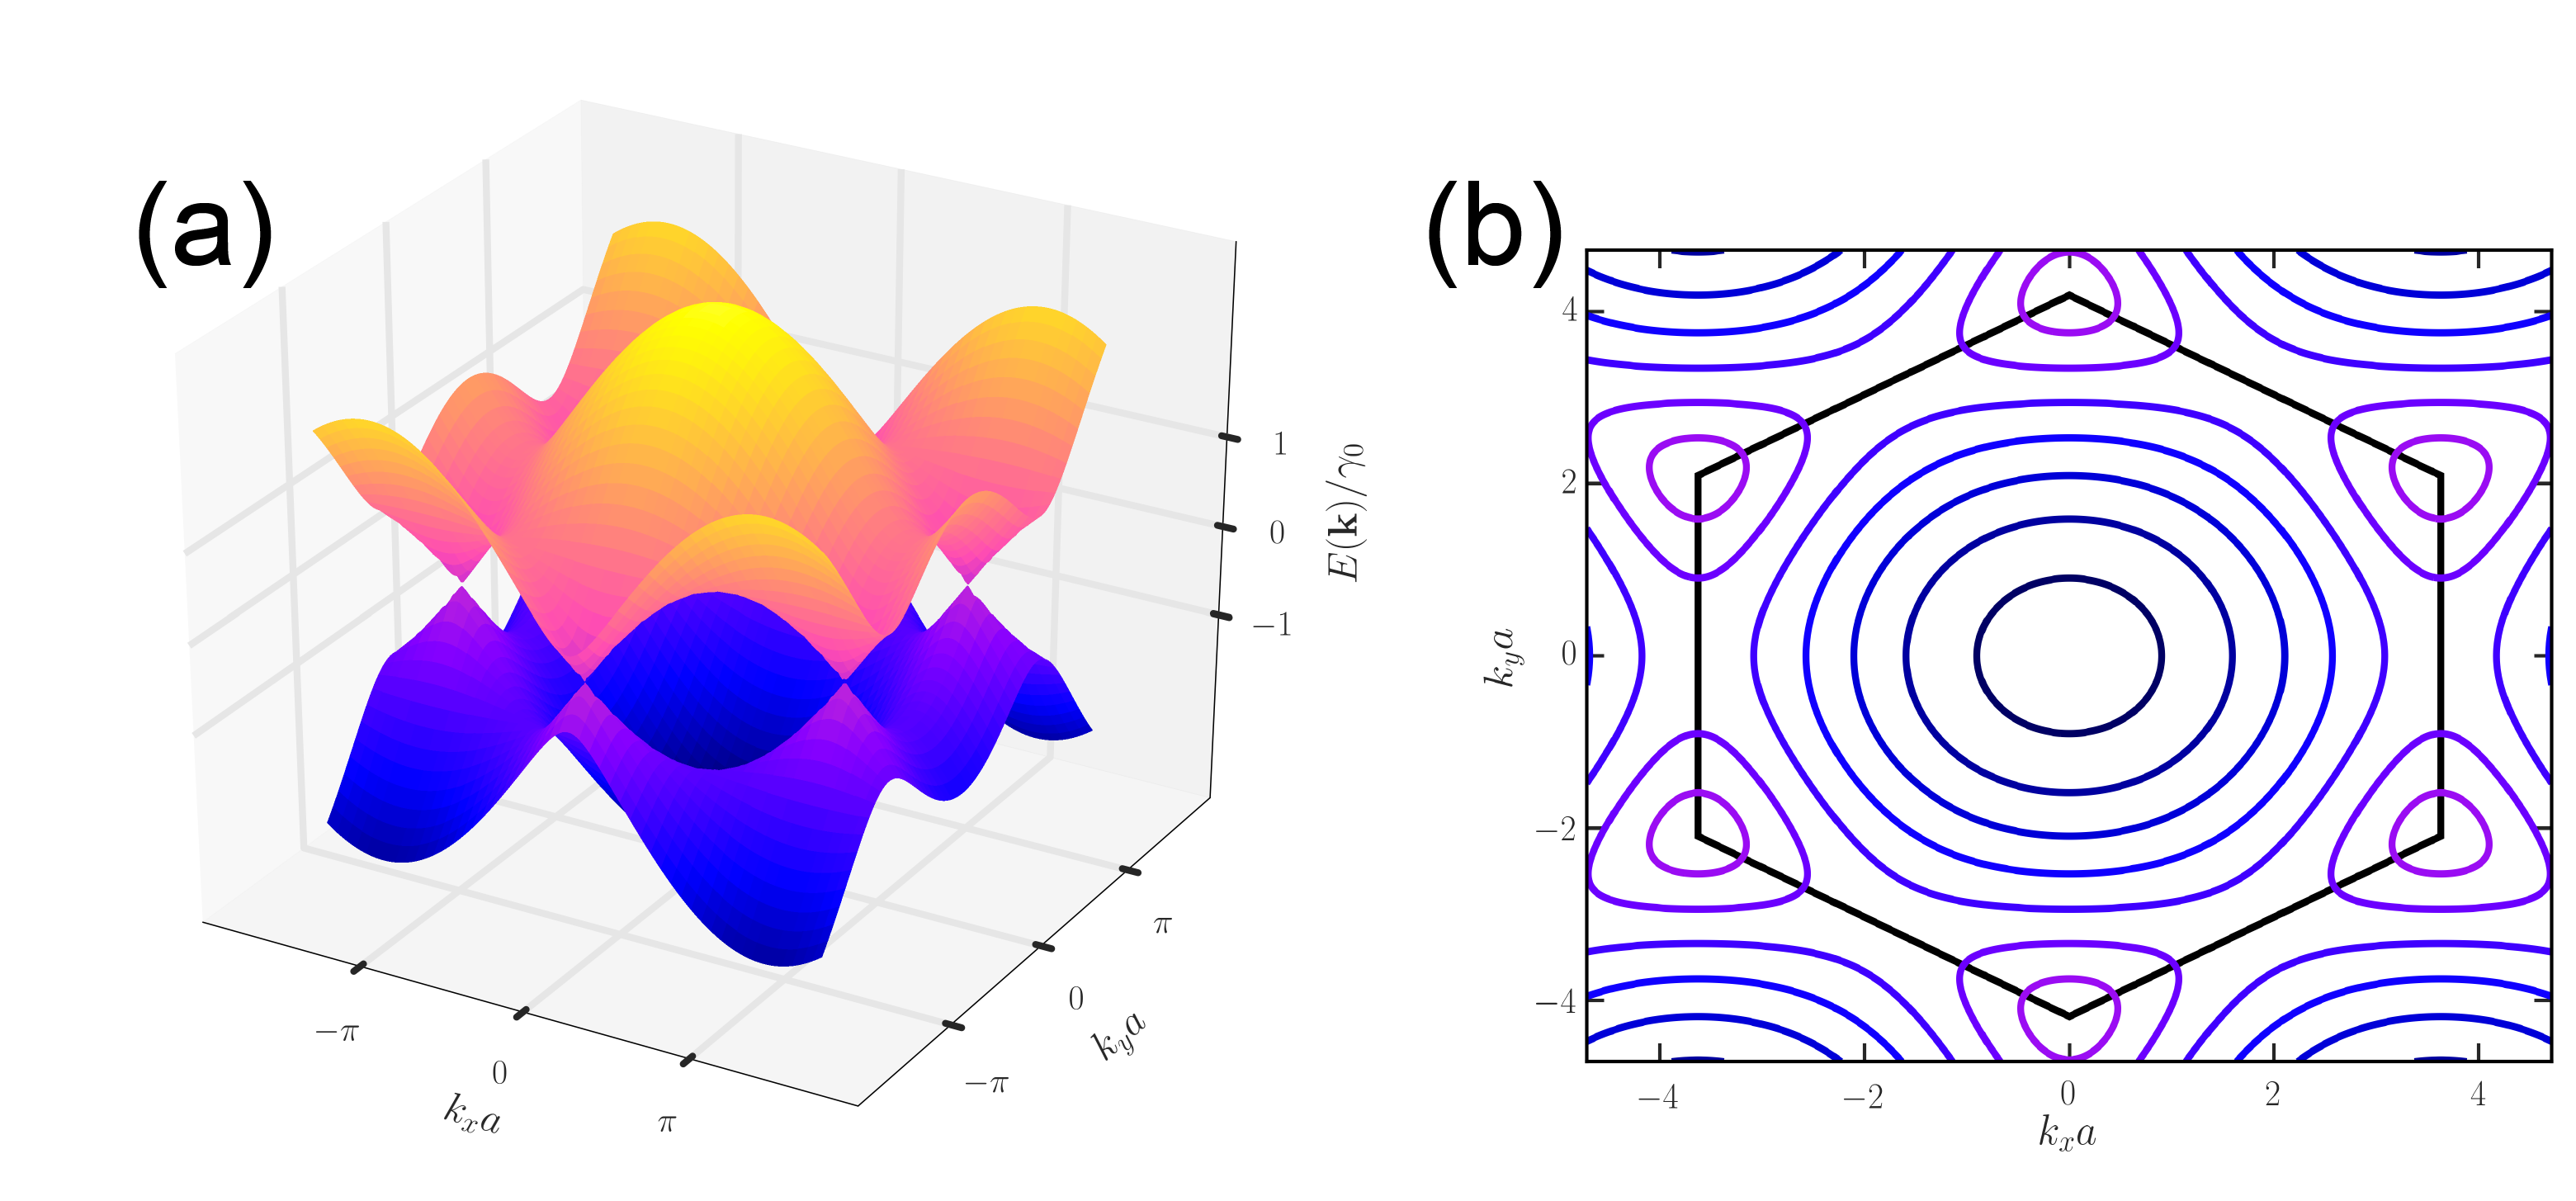
\includegraphics[width = 1.0\textwidth]{chapter2/graphene_band_fig.png}
    \caption{(a) The $\pi$-bands of graphene calculated using a nearest neighbor tight binding model. (b) A contour plot of the lower band with the first Brillouin zone drawn. The bands meet at the three $K$ and three $K'$ points at the vertices of the Brillouin zone.}
    \label{fig:graphene_bands}
\end{figure}

\subsection{Low Energy Bandstructure of Graphene}



\section{Carbon Nanotube Quantum Dots}

How to interpret/understand quantum dot measurements.